\cleardoublepage
\chapter{Implementation??} \label{chap:trans}
\todo[inline,color=red!40]{*1-Introduction}
\todo[inline,color=yellow!40]{*2-Measuring Sensors}
\todo[inline,color=yellow!40]{*3-Real Signal Analysis}

\section{Introduction}
\section{Sensors} %Change latter 
When stimulating a system, by hitting with a hammer on his side surface, the LPG bottle will produce internal vibration, and in this case also produces a sound. For the different amounts of liquid LPG the system will produce a different response in frequency, according to what was stated in the \ref{sec:LPGModel}, this response can be measured with the two different approaches.\\
To capture the sound, the simplest and most obvious approach is to use a microphone for that effect, proceeding with his analysis in frequency. This his one of the easiest approaches, and is going to be used in a first stage to verify the response of the system, in this case it won't be necessary to developed additional hardware, a external microphone is going to be used with this purpose\ref{sec:MIC}.\\

To acquire and measure the vibration, the sensors used must work according to the system mechanical or optical principals of vibration. There is a large variety of sensors that ca be used for that purpose, although there isn't a direct method, or sensor, to measure the vibration and they can be either mechanical or optical. The sensors ca be divided in different groups, based on their behavior they can be active or passive, the type of measurement can be either absolute or relative, and there is also some specific characteristics of the signals that differ from the type of sensor, like the frequency range, signal dynamic and the quality of the data acquired. Sensors are divided in contact and non-contact measurement and subdivided in path/displacement, speed/velocity or acceleration.\\
For contact measurements, sensors related to path/displacement can be potentiometric transmitters or Linear Variable Differential Transmitter (LVDT), to speed/velocity it can be applied the principle of electrodynamics or use a seismometer as a sensor and for acceleration the sensors can be piezoelectric, piezo-resistive, resistive or inductive. In non-contact measurements, path/displacement sensors are eddy current sensors, optical sensors and hall sensors, or can be based on the capacitive principle, for speed/velocity is used a Laser-Doppler vibrometer (LDV) and for acceleration isn't possible to measure directly, although it can be derivate from speed/velocity measurement, but induces a lot of noise in the data acquired\cite{SensorsVibrationMeasurement}\cite{VibrationMeasurementVibration2019}.\\
From all the sensors mentioned, is usually used the contact acceleration to measure the vibration. The use of this types of devices is very wide, as well as the type of accelerometer used and usually the application of them is for monitoring equipment in a reliable way in industry.\\ 
Beside the sensors mentioned, one type of sensors that is commonly used to measure vibrations is the accelerometer, the functioning principle can differ from one to another. The basic principle of a accelerometer is similar to a seismometer, from this there are 3 main types, mechanical, capacitive and piezoelectric. The mechanical is the most similar to a seismometer, with a mass attached to a spring, every time that acceleration occurs, just like in seismometer, the mass moves and a pen attached to the mass traces the vibration captured.
%%Insert here a image to illustrate this
% see in https://www.explainthatstuff.com/accelerometers.html  
Although in the case of the accelerometer, doesn't trace with a pen in paper, instead generates a electrical or magnetic signal. A example of this, is a piezoresistive accelerometer, which has a his mass attached to a potentiometer, and the result of the vibration is a voltage change. When a magnetic variation occurs, usually a hall-effect accelerometer is used for that effect.  
Similar to the mechanical, a capacitive accelerometer, has one of the plates attached to the mass, and measures the capacitance variation, the vibration of capacitance is related with the vibration movement. 
%% Insert another image here
In piezoelectric accelerometers, the quartz crystal is attached to the mass, and the deformation in the piezoelectric material produces a voltage change, correspondent to the vibration movement.
%%Insert here
All the type of accelerometers mentioned have one problem, that is the fact that they aren't practical to use in certain application, as an example a small electronic device. For that, is used the so called MEMS (Micro Electro Mechanical Systems) accelerometers, this type of accelerometer is a combination of electrical and mechanical device, mounted on a silicon chip, this is one advantage of this type of accelerometers, the can be very produced in very small sizes, to allows their application in different types of electronic devices. The functioning of this type of accelerometer can be explained quite easily, an electrode is between two other electrodes, there is a air gap between these two and a small insulation to prevent direct contact between the middle electrode and the other two, on the top and the bottom. The middle electrode is connected with a cantilever, rigid enough to hold his position, but flexible enough to allow the move when the accelerometer moves or tilts, the cantilever is connected to outside of the chip, this is used to measure the difference of capacitance between the middle electrode and the electrodes at the top and at the bottom, the capacitance changes every time the middle electrode moves or tilts.\\
 %%insert the image here as a example, get it from https://www.explainthatstuff.com/accelerometers.html

This type of accelerometers brought important advantages, being their low cost and their small size the most important of it. On the other hand, the use of this devices for condition monitoring is restricted to a small bandwidth, restricted to a few kHz, and it cannot be used to in applications that require lower noise over higher frequency ranges \cite{WhatYouNeed}\cite{HowAccelerometersWork2009}.

%Not that much detail about each type, specially in what concerns about the non contact. Later talk about the accelerometers, and at the end a note and refer the microphone.




\section{Real Signal analysis}\label{sec:MIC}
As mentioned in \ref{subsec:SOAExpRes}, for different LPG bottles, the response to a external impulse will cause different vibration and thus, a different curve in the relation between weight and frequency. So the first step, is to evaluate this relation in the set of LPG bottles available[reference to the image of the bottles], in this case was available 3 LPG bottles, one empty, another half filled and the last completely filled, according to the 80\% rule, with water inside for safety reasons. The easiest way to perform this test is using a microphone, a hammer(or another object to hit the LPG bottle) and MatLab***. To capture the sound produced by hitting the bottle, the microphone of a Phone was used in addition with MatLab to capture the signal and save it in a ".txt" file.
    \subsection*{Signal Capture}
    To use the microphone of the Phone in real time, a App was installed on the Phone and the PC, used to record and save the signal. In this case, the App used is \textit{WO Mic}, available for Android and IOS. In addition on the PC the client application and a virtual device must be installed to use the Phone in the computer to perform any type of tasks, this connection can be made by USB, Bluetooth, Wi-Fi and Wi-Fi Direct.\\
    The software with three components, already mentioned, the \textit{WO Mic App} runs in the Phone, samples the input of the microphone and transmit it to the computer, the \textit{WO Mic Client}, runs in the computer, connect to the app in the phone, and receive the data from the microphone, which is transmitted to the \textit{WO Mic Virtual Device} on which a real microphone device is simulated and provides the audio to any application or program in the computer\cite{WOMicFREE}:\\
    \begin{figure}[!htb]
        \centering
        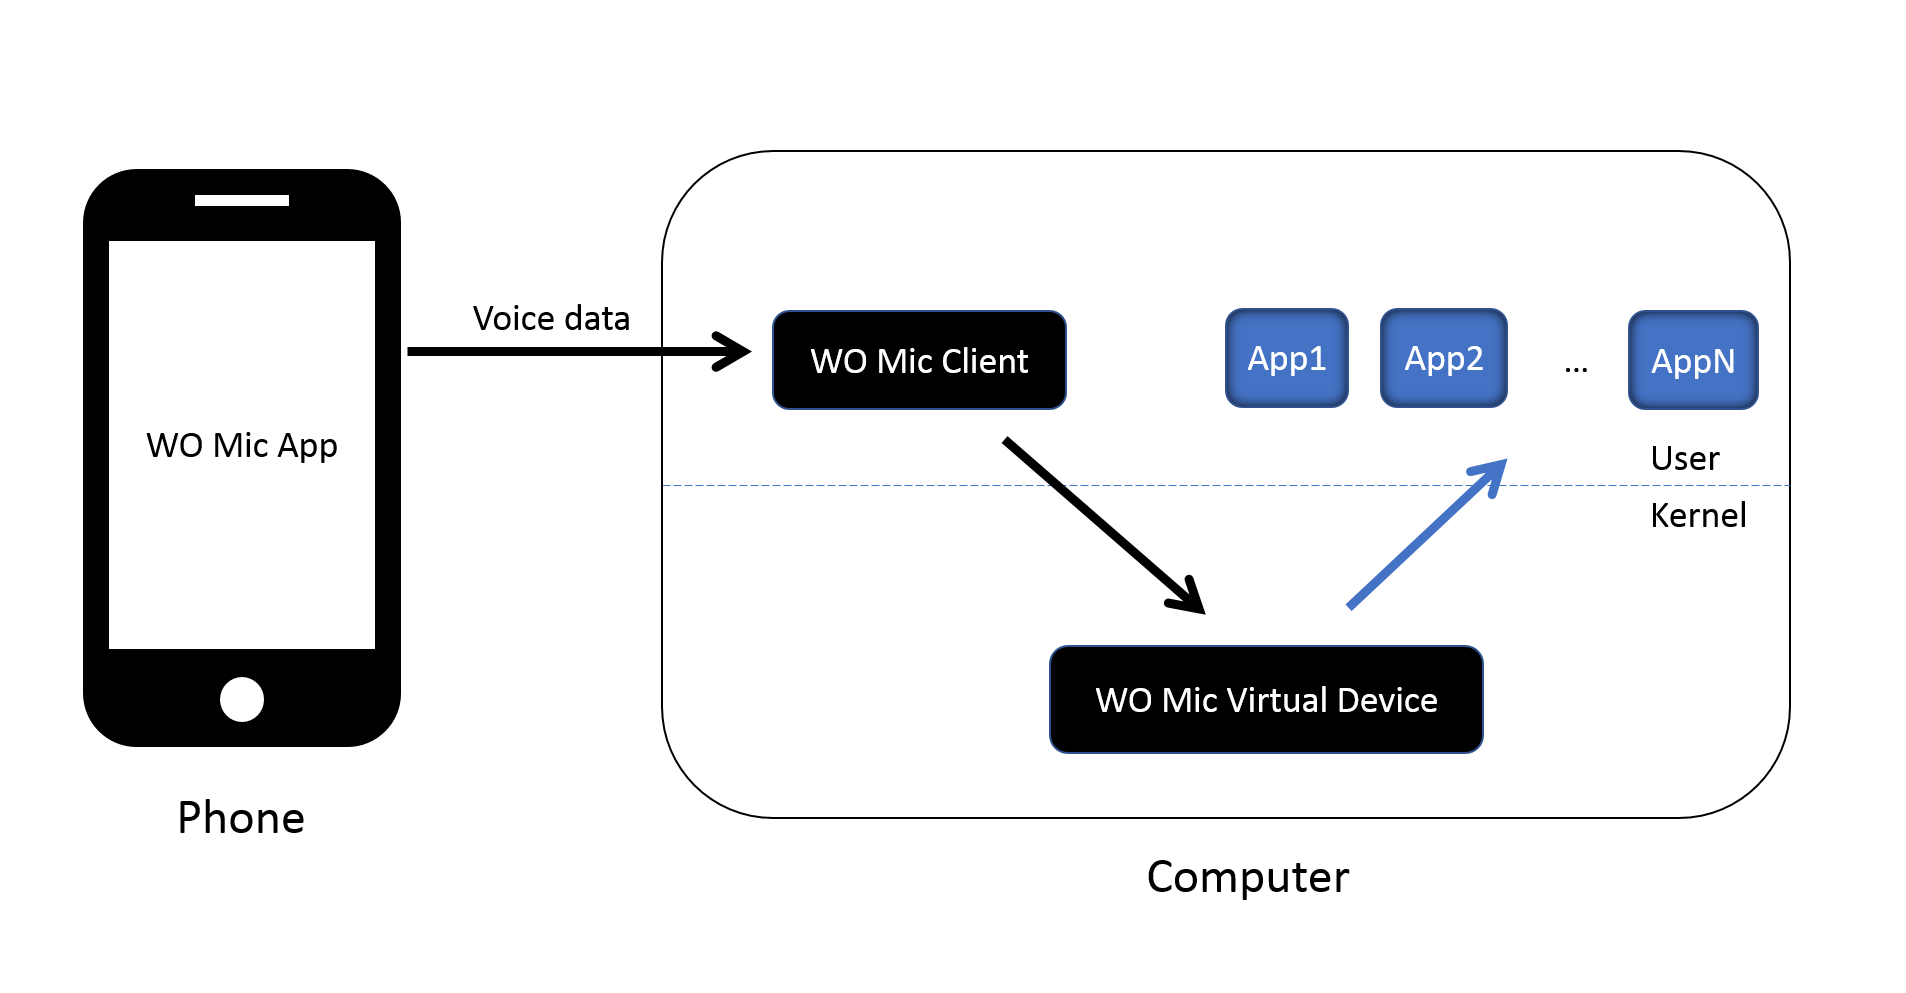
\includegraphics[width=0.65\textwidth]{Chapters/3CHP/Images/WOMICDiag.png}
        \caption{Flow of data in the components of the software\cite{WOMicFREE}}
        \label{fig:diagramWOMIC}
    \end{figure}
    In addition to this, is also necessary to install the drivers of the phone in used, if the connection is made over USB.
    \subsection*{}  

\subsection{Options}
\subsection{Amplifier circuits}
\subsection{Coupling} 

% \begin{figure}[!htb]
%     \centering 
%         \begin{subfigure}[c]{\textwidth}
%             \centering
%             \input{Sections/3Transforms/Images/DFTSymmetry.tex}
%             \caption{}
%             \label{subfig:dft}
%         \end{subfigure}
%         \begin{subfigure}[c]{0.45\textwidth}
%             \centering
%             \input{Sections/3Transforms/Images/DCT1Symmetry.tex}
%             \caption{}
%             \label{subfig:dct1}
%         \end{subfigure}
%         \begin{subfigure}[c]{0.45\textwidth}
%             \centering
%             \input{Sections/3Transforms/Images/DCT2Symmetry.tex}
%             \caption{}
%             \label{subfig:dct2}
%         \end{subfigure}
%         \begin{subfigure}[c]{0.45\textwidth}
%             \centering
%             \input{Sections/3Transforms/Images/DCT3Symmetry.tex}
%             \caption{}
%             \label{subfig:dct3}
%         \end{subfigure}
%         \begin{subfigure}[c]{0.45\textwidth}
%             \centering
%             \input{Sections/3Transforms/Images/DCT4Symmetry.tex}
%             \caption{}
%             \label{subfig:dct4}
%         \end{subfigure}
%         \caption{Sequences generated in the first step of Table \ref{tab:DFTDCT}for the DFT and different DCTs. Filled dots correspond to the original sequence ((a) - \emph{DFT}; (b)) - \emph{DCT-I}; (c)) - \emph{DCT-II}; (d)) - \emph{DCT-III}; (e)) - \emph{DCT-IV}).}
%     \label{fig:2NSeq}
% \end{figure}
% \begin{lstlisting}
%     ./aomenc <INPUT-FILE> -h <HEIGHT> -w <WIDTH> -o <OUTPUT-FILE> --limit=10 -p 1 --cpu-used=8 --i420 --q-hist=64 --end-usage=q --cq-level=<CQ-LEVEL>
% \end{lstlisting}
\clearpage
%\printbibliography[heading=subbibliography]
%\addcontentsline{toc}{section}{References}